%=======================================================================
\section{AMR Component} \label{s:component-amr}
%=======================================================================

Specify data structures and data structure parameters for distributed
AMR hierarchies, such as number of mesh levels, grid patch properties,
rebuild algorithm, dynamic load balancing, refinement criteria, etc.

Hierarchy
Array


\begin{itemize}
\item hierarchy
\begin{item}
\item min\_levels 
\item max\_levels 
\end{item}
\item level
\item grid
\begin{itemize}
\item min\_size
\item max\_size
\item max\_aspect
\item quantum
\end{itemize}
\end{itemize}

\centerline{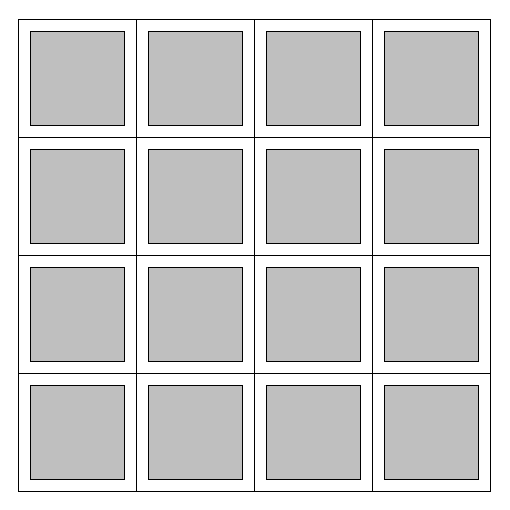
\includegraphics[width=1.8in]{amr4-1.eps} \ \
            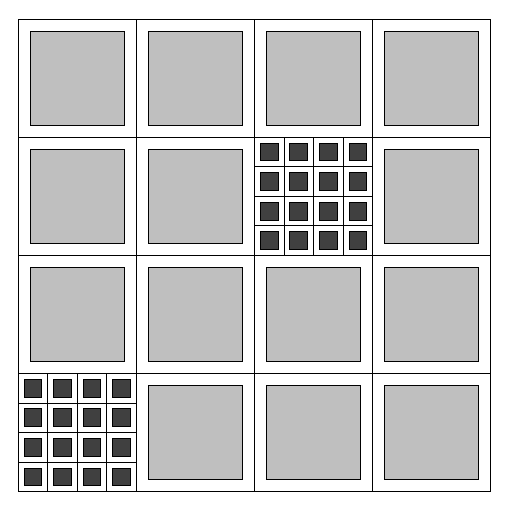
\includegraphics[width=1.8in]{amr4-2.eps} \ \
            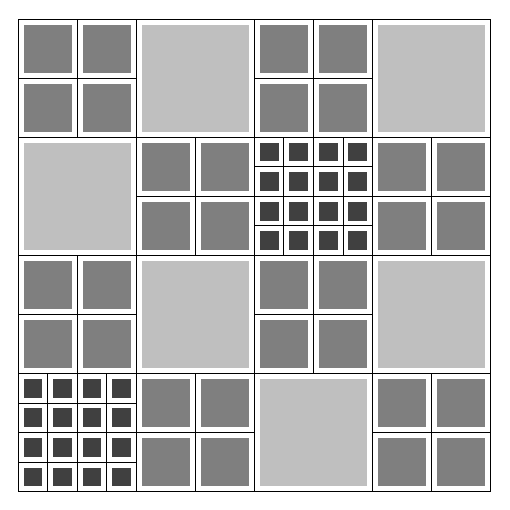
\includegraphics[width=1.8in]{amr4-3.eps}}

\centerline{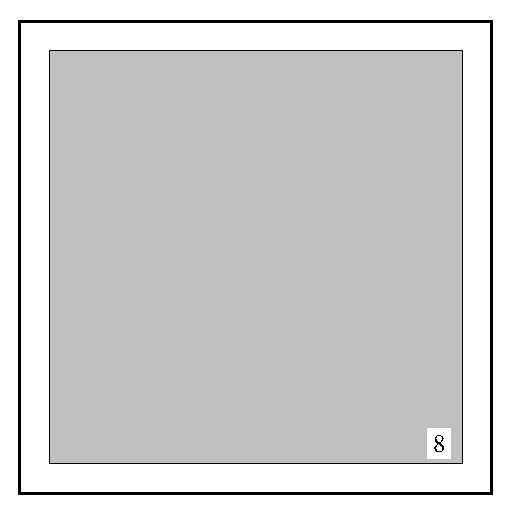
\includegraphics[width=1.8in]{amr2-1.eps} \ \
            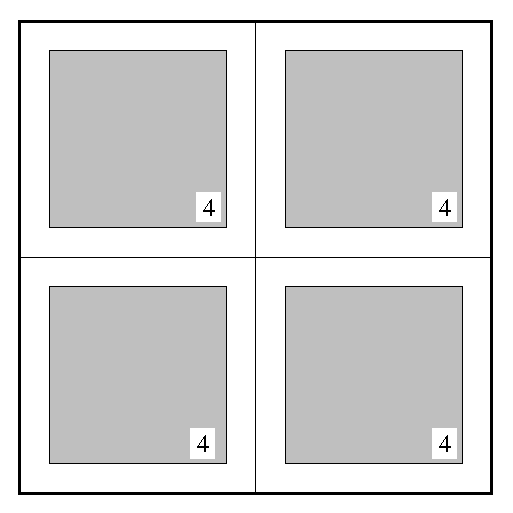
\includegraphics[width=1.8in]{amr2-2.eps} \ \
            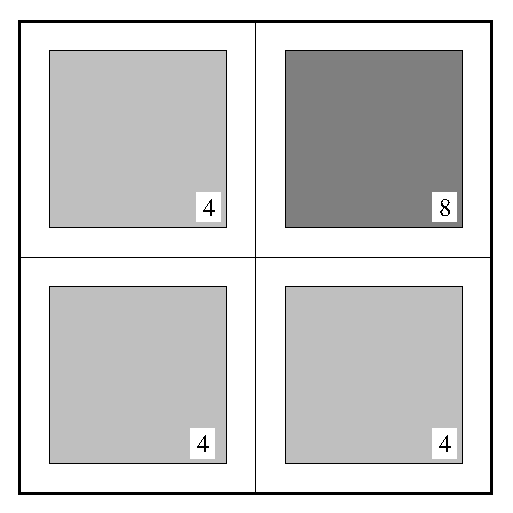
\includegraphics[width=1.8in]{amr2-3.eps}}

\centerline{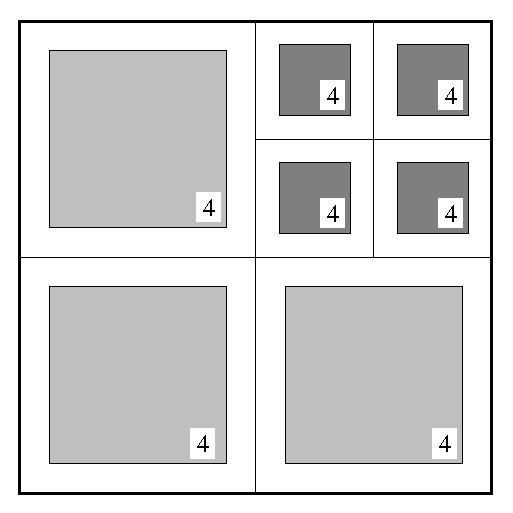
\includegraphics[width=1.8in]{amr2-4.eps} \ \
            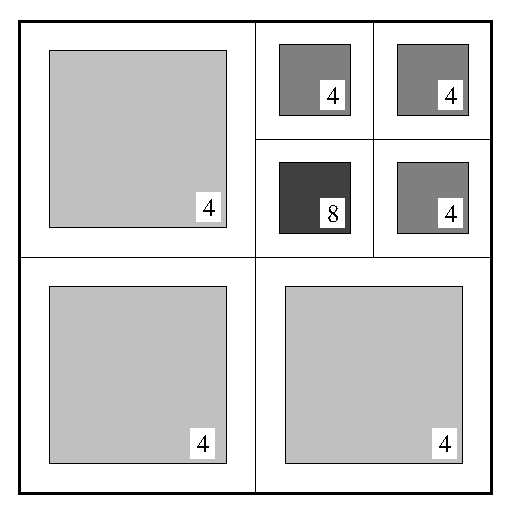
\includegraphics[width=1.8in]{amr2-5.eps} \ \
            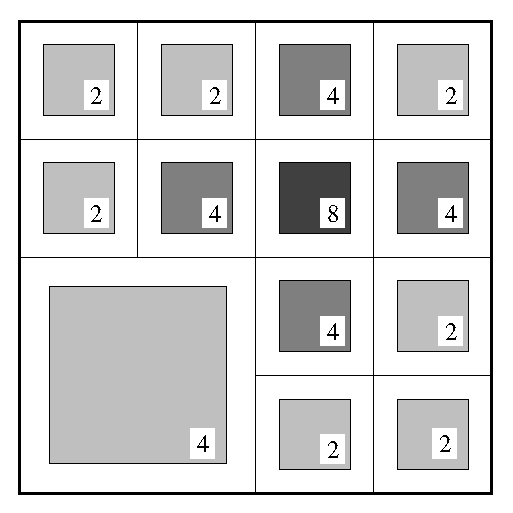
\includegraphics[width=1.8in]{amr2-7.eps}}

\centerline{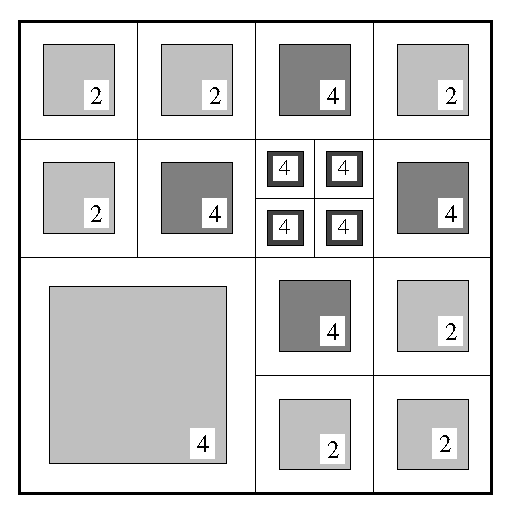
\includegraphics[width=1.8in]{amr2-8.eps} \ \
            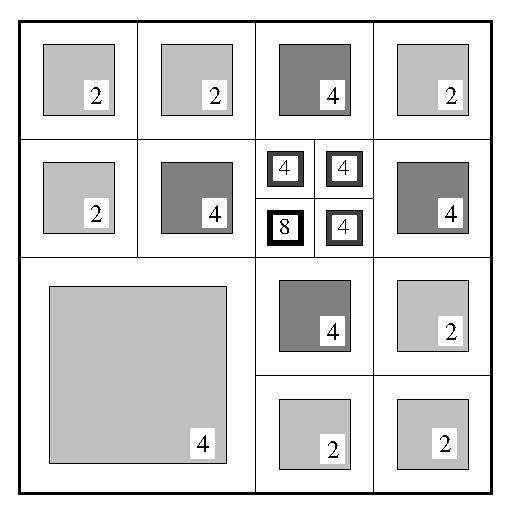
\includegraphics[width=1.8in]{amr2-9.eps} \ \
            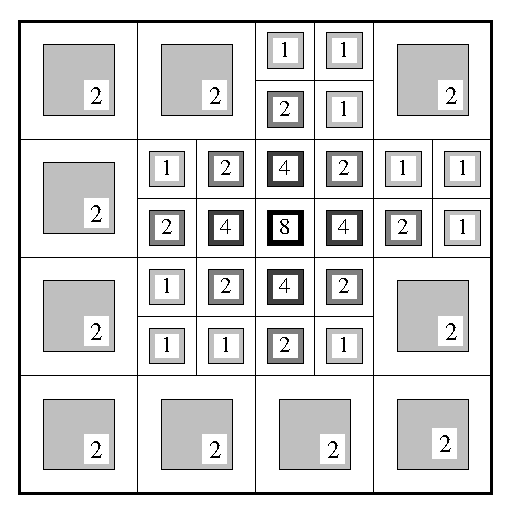
\includegraphics[width=1.8in]{amr2-11.eps}}

%-----------------------------------------------------------------------
\subsection{Use Cases}
%-----------------------------------------------------------------------
%-----------------------------------------------------------------------
\subsection{Parameters}
%-----------------------------------------------------------------------
